\section{Controller}
The Controller is powered by an arduino-knockoff board with an ESP8622 chip already wired in.
The board I used is a LinkSprite D1, which uses the same architecture as a Wemos D1 R1 board (hence the D1 configuration in the platformio project), but you can use any ESP8622 board you want provided that it
\begin{enumerate}
    \item has at least one output pin, and
    \item you can make the necessary connection for sleeping.
\end{enumerate}

\subsection{Power}
\textbf{NOTE: You'll need 2 of these circuits if you're using a small 5V pump.}\\
Unfortuately, the ESP8266 is a power hungry board.
Luckily, we have a way to put the board to sleep so that is stops using so much power.
We only want the board to check in for a few seconds every hour, and in the worst case the board will be running for 5 minutes maybe twice a day\footnote{depending on the plants you're growing}.
The rechargable battery circuit is fairly simple, and uses the following items:
\begin{itemize}
    \item 1 x 3.3V Solar Panel
    \item 1 x 1N4007 High Voltage, High Current Rated Diode
    \item 1 x TP4056 Battery Charger
    \item 1 x 18560 Rechargable Lithium Ion Battery (and holder)
    \item 1 x 0.9V-5V to 5V USB DC-DC Booster
\end{itemize}

The solar panel will essentially charge the battery while the circuit is not in use.
The diode prevents electricty from flowing back through the solar panel, which is important because we only want the solar panel to provide power to the battery, not the other way around.
Since the solar panel provides 3.3V, we use a battery that also provides 3.3V, which is why we need the step up booster.

Below is a diagram showing the basic setup of the power circuit:
\begin{center}
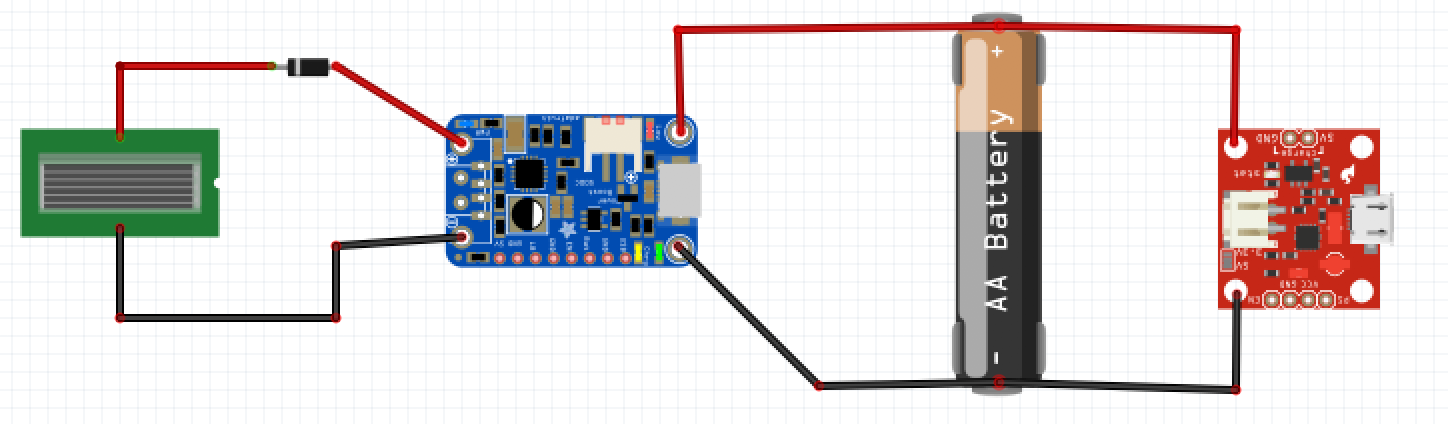
\includegraphics[width=\textwidth]{controller/solar-circuit.png}
\end{center}
The USB cable will come out of the red component and into whatever component needs power.

\subsection{Relay Circuit}
A relay is a component that allows you to stop or start the flow of electricity through the system.
You control it by sending a HIGH signal to the SIG pin on the relay.
This is easy enough to do on the arduino; on the software side, we will just use a \texttt{digitialWrite(outputPin, HIGH)} to switch the relay on.
Below is a diagram of the board conencting into the relay\footnote{I had to use an UNO here to represent the board, but just imagine any ESP8266 board here. Also, the white disk represents the power source.}:
\begin{center}
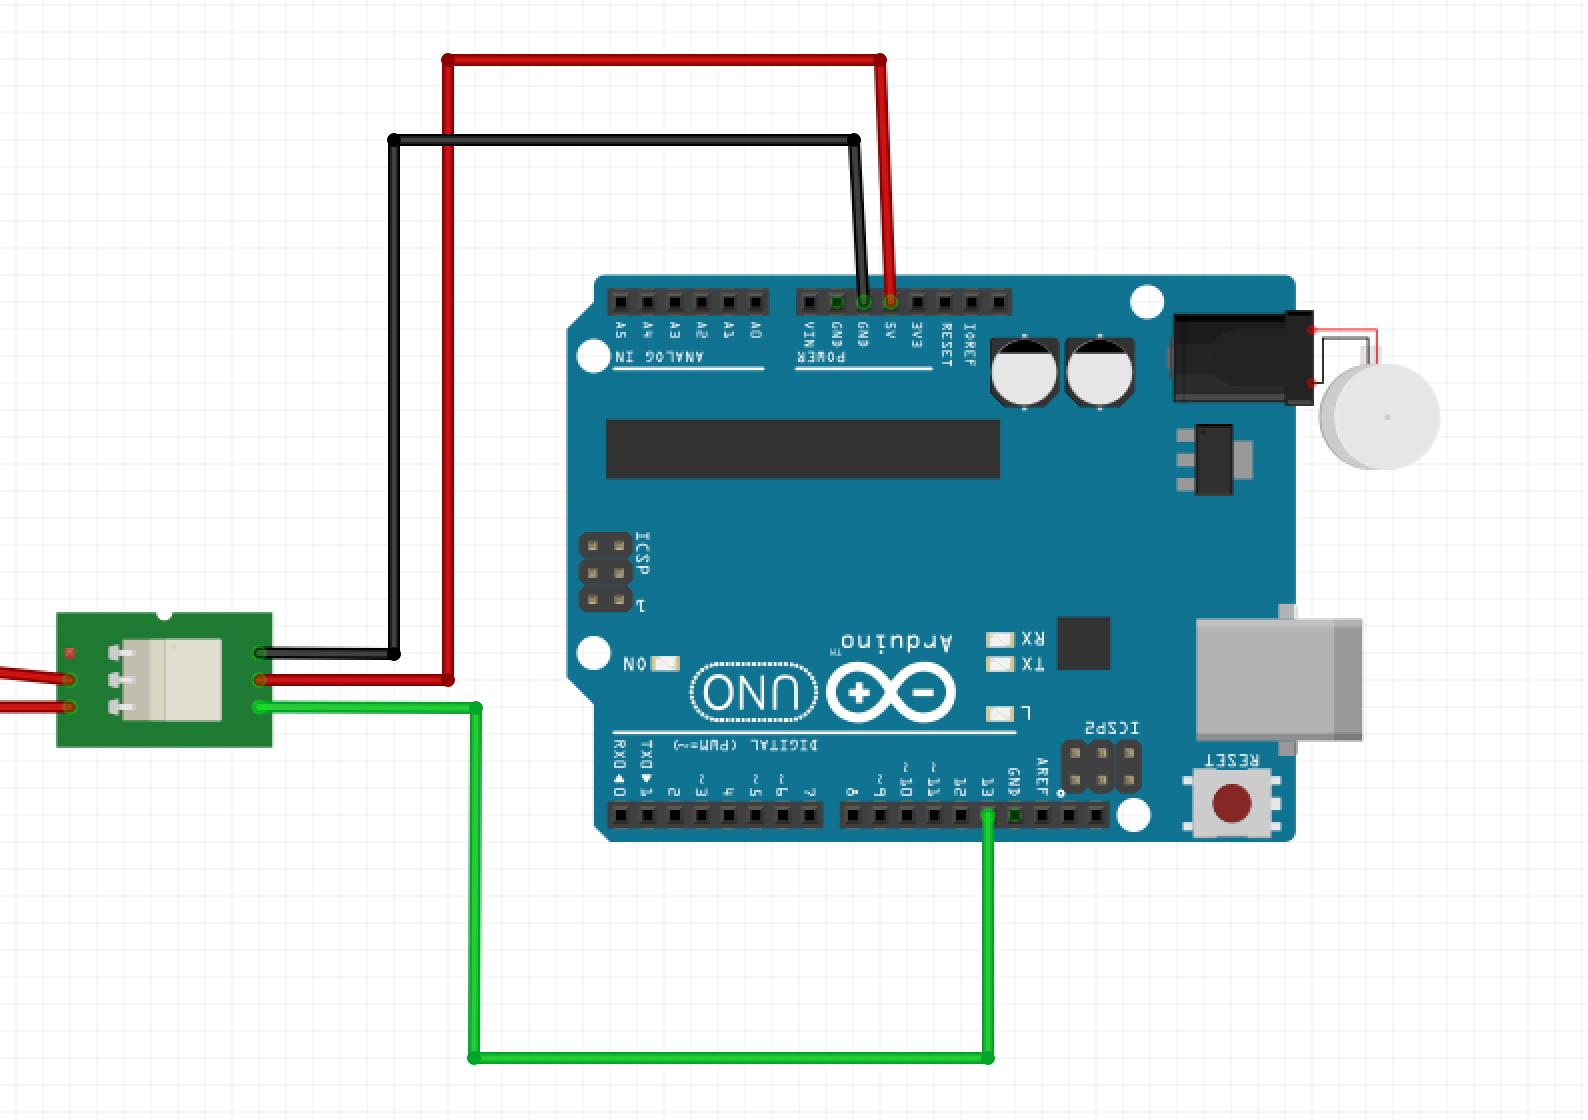
\includegraphics[width=0.5\textwidth]{controller/controller-circuit.png}
\end{center}

On the other side of the relay, we'll need to connect a power source to the NO (normally open) pin, and connect the VCC for the pump to the C (common) pin, and then run the GND of the pump to the GND of the power supply.
We want to use the NO pin of the relay because in that configuration, the default state is ``off''.
The third pin on that side of the relay is NC (normally closed), and it would cause the circuit to default to ``on''.

Below is a diagram of only the relay setup for the pump\footnote{Unfortuately, Fritzing doesn't have a pump object, so I've used a potentiometer object here to represent it. Also, the power supply is represented by the white disk.}:
\begin{center}
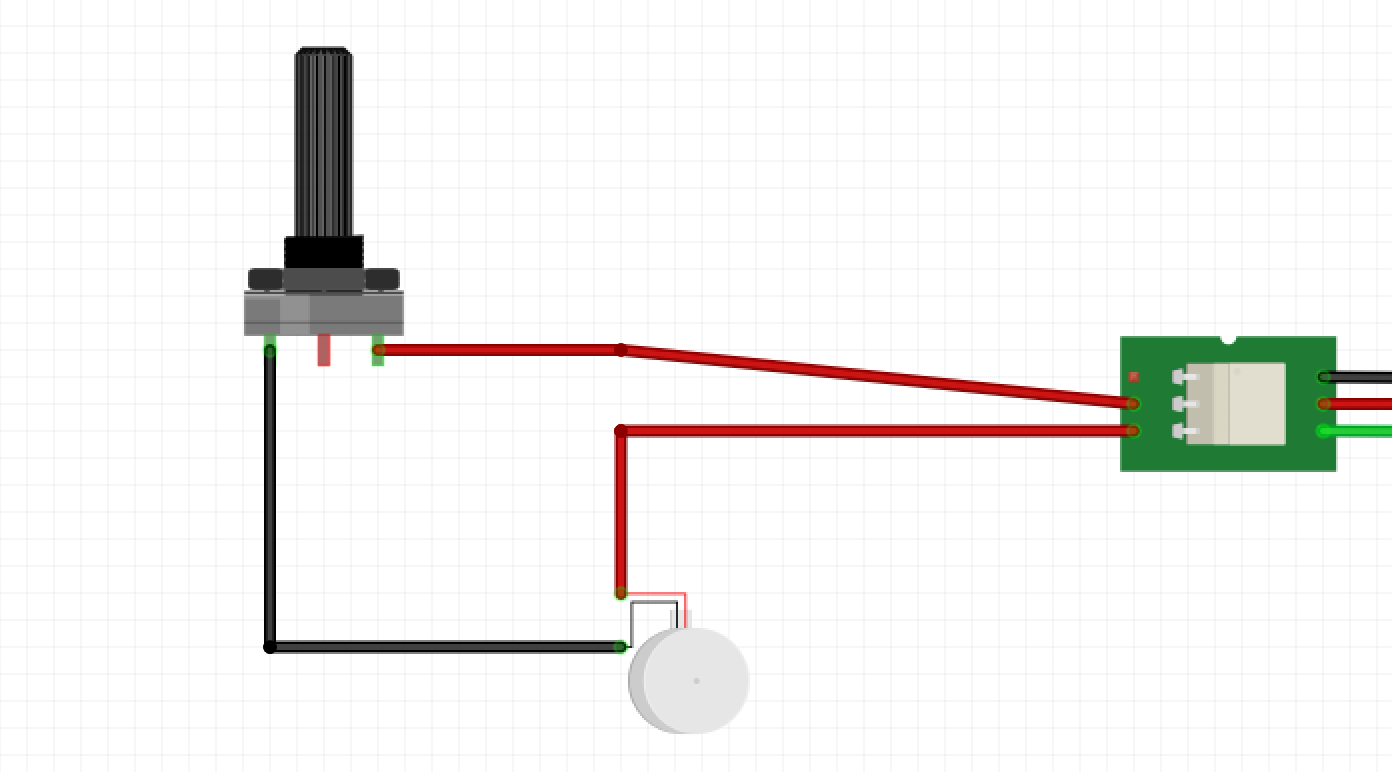
\includegraphics[width=0.5\textwidth]{controller/pump-circuit.png}
\end{center}

